\documentclass{article}
\usepackage[utf8]{inputenc}
\usepackage{amsmath}
\usepackage{mathtools}
\usepackage{bm}
\usepackage{graphicx}
\usepackage{float}

\usepackage{rotating}

\title{COL352: Assignment 4}
\author{Sachin 2019CS10722 \\
        Saurabh Verma 2019CS50129\\}
\date{March, 2022}

\begin{document}
\maketitle

\section{Question 1}
\textbf{Show that every infinite Turing-recognizable language has an infinite decidable subset.}\\
\newline 
\textbf{Given:} So lets us assume that the turing-recognizable language to be L. As we know a language is turing-recognizable iff it as an enumerator which accepts it. Let that enumerator be W. \\
\textbf{Proof Idea:} We will give a new language M which will be the subset of the language A and would be also infinite. Then we will that we could construct a TM T which would accept it. Also we will show that the TM constructed is a decider. So thus we would have proved the above stated hypothesis. \\
\textbf{Proof:} Let us give the description of the new language M. So string $w \in M$ iff it satisfies the following given properties:
\begin{enumerate}
    \item The enumerator W should have printed this string for number of times greater than 0.
    \item $|w|$ should be grater than the length of all the individual strings W has printed before. 
\end{enumerate}
So we have got the description of the language M. Now clearly $M \subseteq L$, because L is the set of all the strings printed by W and M is set of strings printed by W with some extra conditions.\\
Also M is an infinite set. To show this let us take any $k \geq 0$. We know this that there are only finitely many strings which are possible than the length k. So it is bound to happen that the enumerator W will print a string greater than k. Let the first string printed whose length is greater than k be q. Clearly q belongs to the set M as it satisfies both the conditions required. Now L is an infinite set so k can be any arbitrary number. This means that A would contain strings whose lengths are arbitrary long. Thus the set A is infinite. \\
Now we have shown that language A is infinite and subset of M. we just have to create a TM T for the language A and show it is a decider. So on every input w the TM T follows the following steps in order:
\begin{enumerate}
    \item We run the enumerator W repeatedly till the point it either prints the string w or prints a string whose length is greater than $|k|$.
    \item If the length of string printed is greater than $|k|$ reject. 
    \item If the printed string is w accept.
\end{enumerate}
Now we have to show T decides A. Firstly we can see that T always halts on any input. This is due to the fact that enumerator E is continously printing string of L which is an infinite set with arbitrary long strings. So the machine would come of out of step 1 after some time. And if it came out it will either reject or accept. Hence the machine always halts.\\
Now we have to show that for any string w the following thing holds $w \in M$ iff T accepts it. Now if we take a string $w \in M$ clearly T would accept as the very conditions (1 and 2 mentioned on the previous page) that made w to be in M is what the T is checking. Also the other way is clear too. If a string is accepted by T that clearly implies both the conditions of being in M is satisfied. So in total we can say T decides M.\\
We have shown  a decidable infinite subset of the infinite recognizable language. 
Hence Proved.

\pagebreak

\section{Question 2}
\textbf{Show that single-tape TMs that cannot write on the portion of the tape containing the input string recognize only regular languages.}\\
\newline 
\textbf{Given:} So we are given a single taped TM T= $(Q, \Sigma, \Gamma, q_0, q_a, q_r)$ ($q_a$ is accept state and $q_r$ is the reject state) with the restriction that it can not write on the input portion on the tape. Let the language recognized by such a TM be L. Now we have to show that language L is in-fact regular. \\
\textbf{Proof Idea:} Now we have to show that L is regular. To do so we will show a myhill-nerode relation on the language.\\
Now let us see what is the difference between the TM given to us and the normal one. One important point is that the input tape in T has two part one is only the readable part(which has the input string) and the readable-writable part which is initially blank. Here in the present setting the problem is the restriction on the what the TM can remember (as the only way it has to remember is to write it down on the tape or through states). When T transitions from the input region of the tape to writable region, it cant remember(as it cant write) any information other than the state it is in. Same thing happens when it enters back into the input region, it only know the state and nothing of the things written on the writable region. So in a way the state that T emerges out of read only region is the only memory T has of the input. This exact fact is used by us to prove that T recognises only regular languages. \\
\textbf{Proof:} As described above T can only remember certain information about the input. The fact that T can not remember what it has written in the writable region gives rise to a function which is unchanging, we will define it as $f(w,q)=q'$. The meaning of this function is that when the input head enters the input region on state q, the input region has w, then T would leave the input region on the state q'. Now let us take care of few technicalities. First if after entering the input region if the input head doesn't leave the input region then q' would be equal to $q_a$ or $q_r$ according to the fact that w is accepted or not. Now we will show that this function remains constant throughout the run of the machine. This is because of the fact that since T cannot write in the input region w remain constant. Also this function does not have any effect by what is written in the writable region of the tape, and this should be the case as T cant reference any of that in the read-only region.\\
So when describing this function it would lead to a table with $|Q|$ entries. We have to add one more entry to this which is the state which is reached when the input head moves into the writable region for the first time(This is not captured in the function entries given up until this point because it is the first entry to the writable region.). If the input head never moves into the writable region this entry must be $q_a$ or $q_r$ accordingly. Now lets call this entry $f(w, \epsilon)$ \\
This function completely determines the behaviour of T on the input string w. This is due to again the fact of restricted memory present in this model.\\
Now lets define the myhill-nerode relation on any two strings a and b , $a \equiv b$ iff all the entries of the table of a and b is the same. Now we will show that this relation satisfies all the properties required. 
\begin{itemize}
    \item \textbf{Finite Index:} Now let us look at the size of the table. The number of rows in the table is exactly equal to $|Q|+1$ and for each of these rows the possible entry set size if $|Q|$. So the number of different table could be only as large as ${|Q|^{|Q|+1}}$. Now number of equivalence classes of this relations is  finite.
    \item \textbf{Refinement:} Now the refinement property states that if x and y belong to the same equivalent class then they are either both rejected or both accepted. Now this is clearly the case. This is due to the fact that this table completely determines all that T does on the input. In the table we fill $q_a$ or $q_r$ at some rows too if the input head doesn't return to the writable region(described above). If the table is same then that means that they are both either rejected or accepted.
    \item \textbf{Right Congruence:} The right congruence property states that if x and y belong to same class then so do xz and yz. So in our case it would mean that the tables of both xz and yz is also the same. This is easy to verify. Since table of x and y was initially same and now identically we have added a alphabet z at the end of it the changes to the table would be also identical. 
\end{itemize}
Now since we have shown a myhill-nerode relation on the language L this means that L is regular. Thus the language recognized by single-tape TMs that cannot write on the portion of the tape containing the input string is regular. Hence Proved.

\pagebreak


\section{Question 3}

\textbf{Let C be a language. Prove that C is Turing-recognizable iff a decidable language D exists
such that
    \begin{center}
        $C = \{x | \exists y (<x, y> \in D) \}$\\
    \end{center}
}

\pagebreak


\section{Question 4}

\textbf{Say that a variable A in CFL G is usable if it appears in some derivation of some string
w $\in$ G. Given a CFG G and a variable A, consider the problem of testing whether A is
usable. Formulate this problem as a language and show that it is decidable\\}

\pagebreak


\section{Question 5}

\textbf{Consider the problem of determining whether a Turing machine M on an input w ever at-
tempts to move its head left when its head is on the left-most tape cell. Formulate this
problem as a language and show that it is undecidable\\}

To prove that a language is undecidable it is sufficient to show that if it were decidable then it would imply
that some other language that is already known to be undecidable is also decidable.\\
We will follow the similar proof by contradiction and assume language L to be decidable.\\
First let us provide a formal desciption of L:\\
$L = \{ <M,w> | $ M moves its head left on w when its head is on the left-most tape cell $ \}$\\

Now, assume L to be decidable. Then there exists a turing machine T that decides L.\\
Let us try to construct a turing machine T' from T that accepts $A_{TM}$ (that is what we are doing in every undecidablility proof in class)
\begin{enumerate}
    \item Run M on w and if at any transition it accpets w, move to leftmost tape cell and try to move its head to left.\\
        This is done to make sure that on acceptance there is left movement of the head on leftmost tapecell.\\
    \item If at any non accepting transition tape is on leftmost cell and try to move left, then move rightward (writing the same character that M wanted to write on this transition) and move 
            left without changing tape. More formally:- \\
            $q_iw_1....w_k \rightarrow q_iw'_1...w_k $\ is changed to $q_iw_1....w_k \rightarrow w'_1q_iw_2...w_k \rightarrow q_1w'_1....w_k$\\
            This is done to make sure that there if no left movement if head is on leftmost tape, if state is not accepting.
\end{enumerate} 

Using above construction we've made sure that T' attempts to move its head left from leftmost tapecell on $<M,w>$ if and only if M accepts w.\\
Now, simply run T' on T to decide whether it attempts to move its head left from leftmost tapecell. That way we can decide whether M accepts w or not but that is 
a contradiction since $A_{TM}$ is undecidable (proved in class)\\
Hence L is undecidable.

\pagebreak


\section{Question 6}

\textbf{Consider the problem of determining whether a Turing machine M on an input w ever at-
tempts to move its head left at any point during its computation on w. Formulate this
problem as a language and show that it is decidable.\\}

The language formed by the above problem is:- \\
$L = \{ <M,w> |$ M moves its head left on w at any point \}.\\

To prove that any language is decidable it is sufficient to show that there exists a Turing Machine that 
decides that language. So we will construct a turing machine T that can decide the above language.\\
But before that let's analyse the 2 possible cases of w on M:-

\begin{enumerate}
    \item \textbf{M never moves its head left on w :}
    This means that M always moves its head right on w. Lets see the run of T on w (Let $|w| = n$).\\
    $q_0w \rightarrow aq_1w_2....w_n \rightarrow_* w'q_i \sqcup \rightarrow w' b q_{i+1} \sqcup \rightarrow_{k-1} w' b_1....b_k q_{i+k} \sqcup   $\\
    Now, since number of states and n are finite, if we take k big enough by pegionhole principle $q_{i+k} = q_i$.\\
    Take k = $|Q|+1$ $=>$ by pegionhole principle some of the states will repeat in k transitions, and since next tape alphabet 
    is always $\sqcap$ (since we are always moving right) same cycle will repeat infinite times.\\
    Hence if M don't moves its head left on w in first $|w| + |Q| + 1$ transitions then it will never move its head left on w.\\

    \item \textbf{M moves its head left on w :}
    From the above case it is clear that M moves its head left on w in first $|w| + |Q| + 1$ transitions.\\
    
\end{enumerate}

Now consider the desciption of T on w.\\
\begin{enumerate}
    \item Run first $|w| + |Q| + 1$ transitions of M on T.
    \item If at any time M moves its head left on w then accept.
    \item Otherwise reject.
\end{enumerate}


Point 1 is possible because we can always simulate a turing machine on another turing machine if its description is given (Universal Turing machine).\\
Correctness of the above description is proved earlier by the claim that f M don't moves its head left on w in first $|w| + |Q| + 1$ transitions then it will never move its head left on w.\\
\pagebreak


\section{Question 7}

\textbf{Let $AM_{BCFG} = \{< G > | G$ is an ambiguous CFG $\}$ \\
    Show that $AM_{BCFG}$ is undecidable via a reduction from PCP\\}

To prove that $AM_{BCFG}$ is undecidable first we will assume that $AM_{BCFG}$ is decidable. Then 
we will try to arrive at contradiction by showing that this would imply PCP is decidable but that is not.\\

First let's see an instance P of PCP:- \\

Provided:\\
$\lfloor \frac{t_1}{r_1} \rfloor , \lfloor \frac{t_2}{r_2} \rfloor ....... \lfloor \frac{t_n}{t_n} \rfloor$ \\
where, $t_i , r_i \in \Sigma^* , |t_i| = |r_i| \forall i \in [1,n]$\\

Find:\\
a sequence $\{ i_1,i_2.....i_k \}$ such that $t_{i_1}t_{i_2}.....t_{i_k} = r_{i_1}r_{i_2}.....r_{i_k}$\\

Now, we need to create a grammar G from P such that deciding whether G is  ambiguous or not would solve PCP P.\\
For any grammar to be ambiguous it have some string w that has 2 left most derivations.\\
So, we need to match solution of P to existence of w.\\

One such construction is as follows:- \\

G = $\{ V,\Sigma, R, S \}$, where \\
$Q = \{S, T, R\}$\\
$\Sigma = \{t_1, t_2 .... t_n\} \bigcup \{r_1, r_2 .... r_n\} \bigcup \{1,2,....n\}$\\
R defined as follows:- \\
$S \rightarrow T | R$\\
$T \rightarrow t_iTi | t_i i :  \forall i \in [1,n] $\\
$R \rightarrow r_iRi | r_i i :  \forall i \in [1,n] $\\

Now, suppose $AM_{BCFG}$ is decidable. Then we can decide whether G is ambiguous or not:- \\
Suppose G is ambigious.\\
$=> \exists w \in \Sigma^* $ such that w has 2 left most derivations\\
following cases are possible:- 

\begin{enumerate}
    \item \textbf{First production rule for w is same in its both derivations: }\\
    We will shoe that this is not possinle.\\
    WLOG let it be $S \rightarrow T$ (since both $S \rightarrow T , S \rightarrow R$ have equivalent further production rules in T and R and proof for one can be 
    easily converted to other, so we will prove ony for one of them) \\

    Parse trees formed are:- \\  

    \begin{figure}[H]
        \centering
        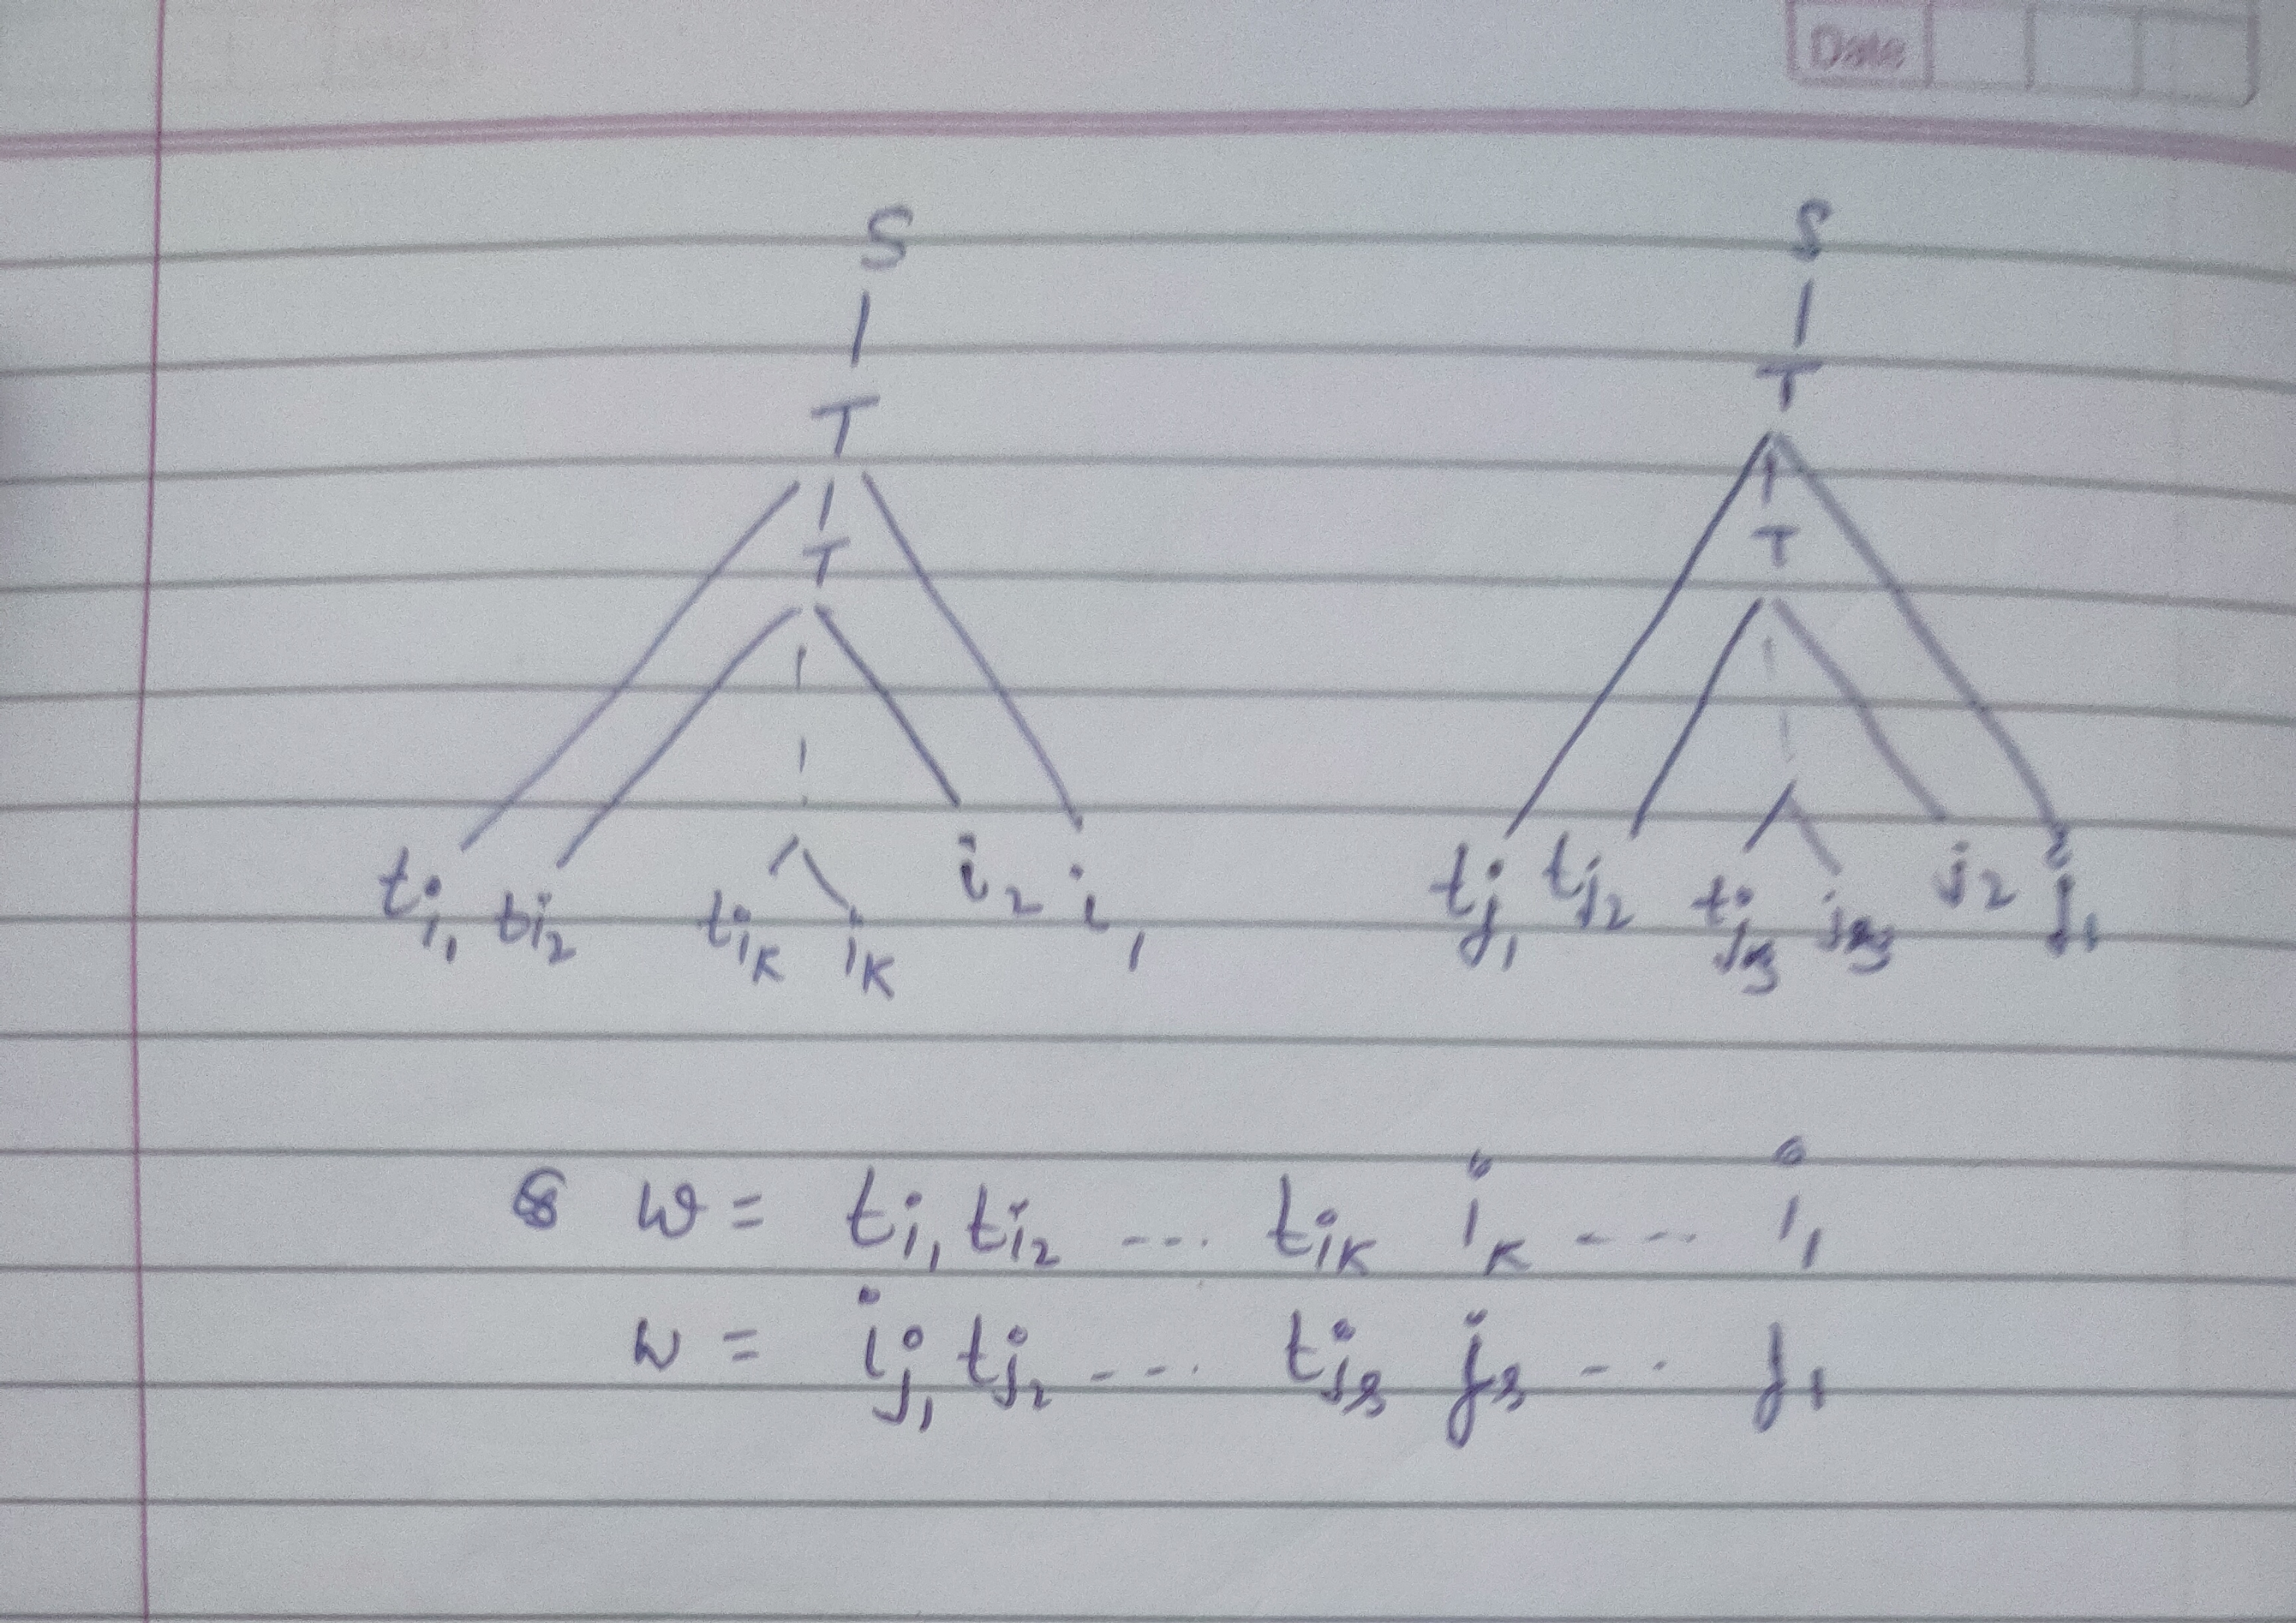
\includegraphics[width=7cm]{1.jpg}
    \end{figure}

    We have w = $t_{i_1}t_{i_2}....t_{i_k}i_k....i_1$ = $t_{j_1}t_{j_2}....t_{j_s}j_s....j_1$\\
    Since i's and j's are unique characters, matching both of them from last would yield $i_1 = j_1 ..... i_k = j_s$\\
    That gives both of the derivations are same. \\
    Hence this case is not possible.\\

    \item \textbf{First production rule for w is different in its two derivations:}\\
    So, only possible different production rules are $S \rightarrow T, S \rightarrow R$\\
    Parse trees formed are:- \\  
    
    \begin{figure}[H]
        \centering
        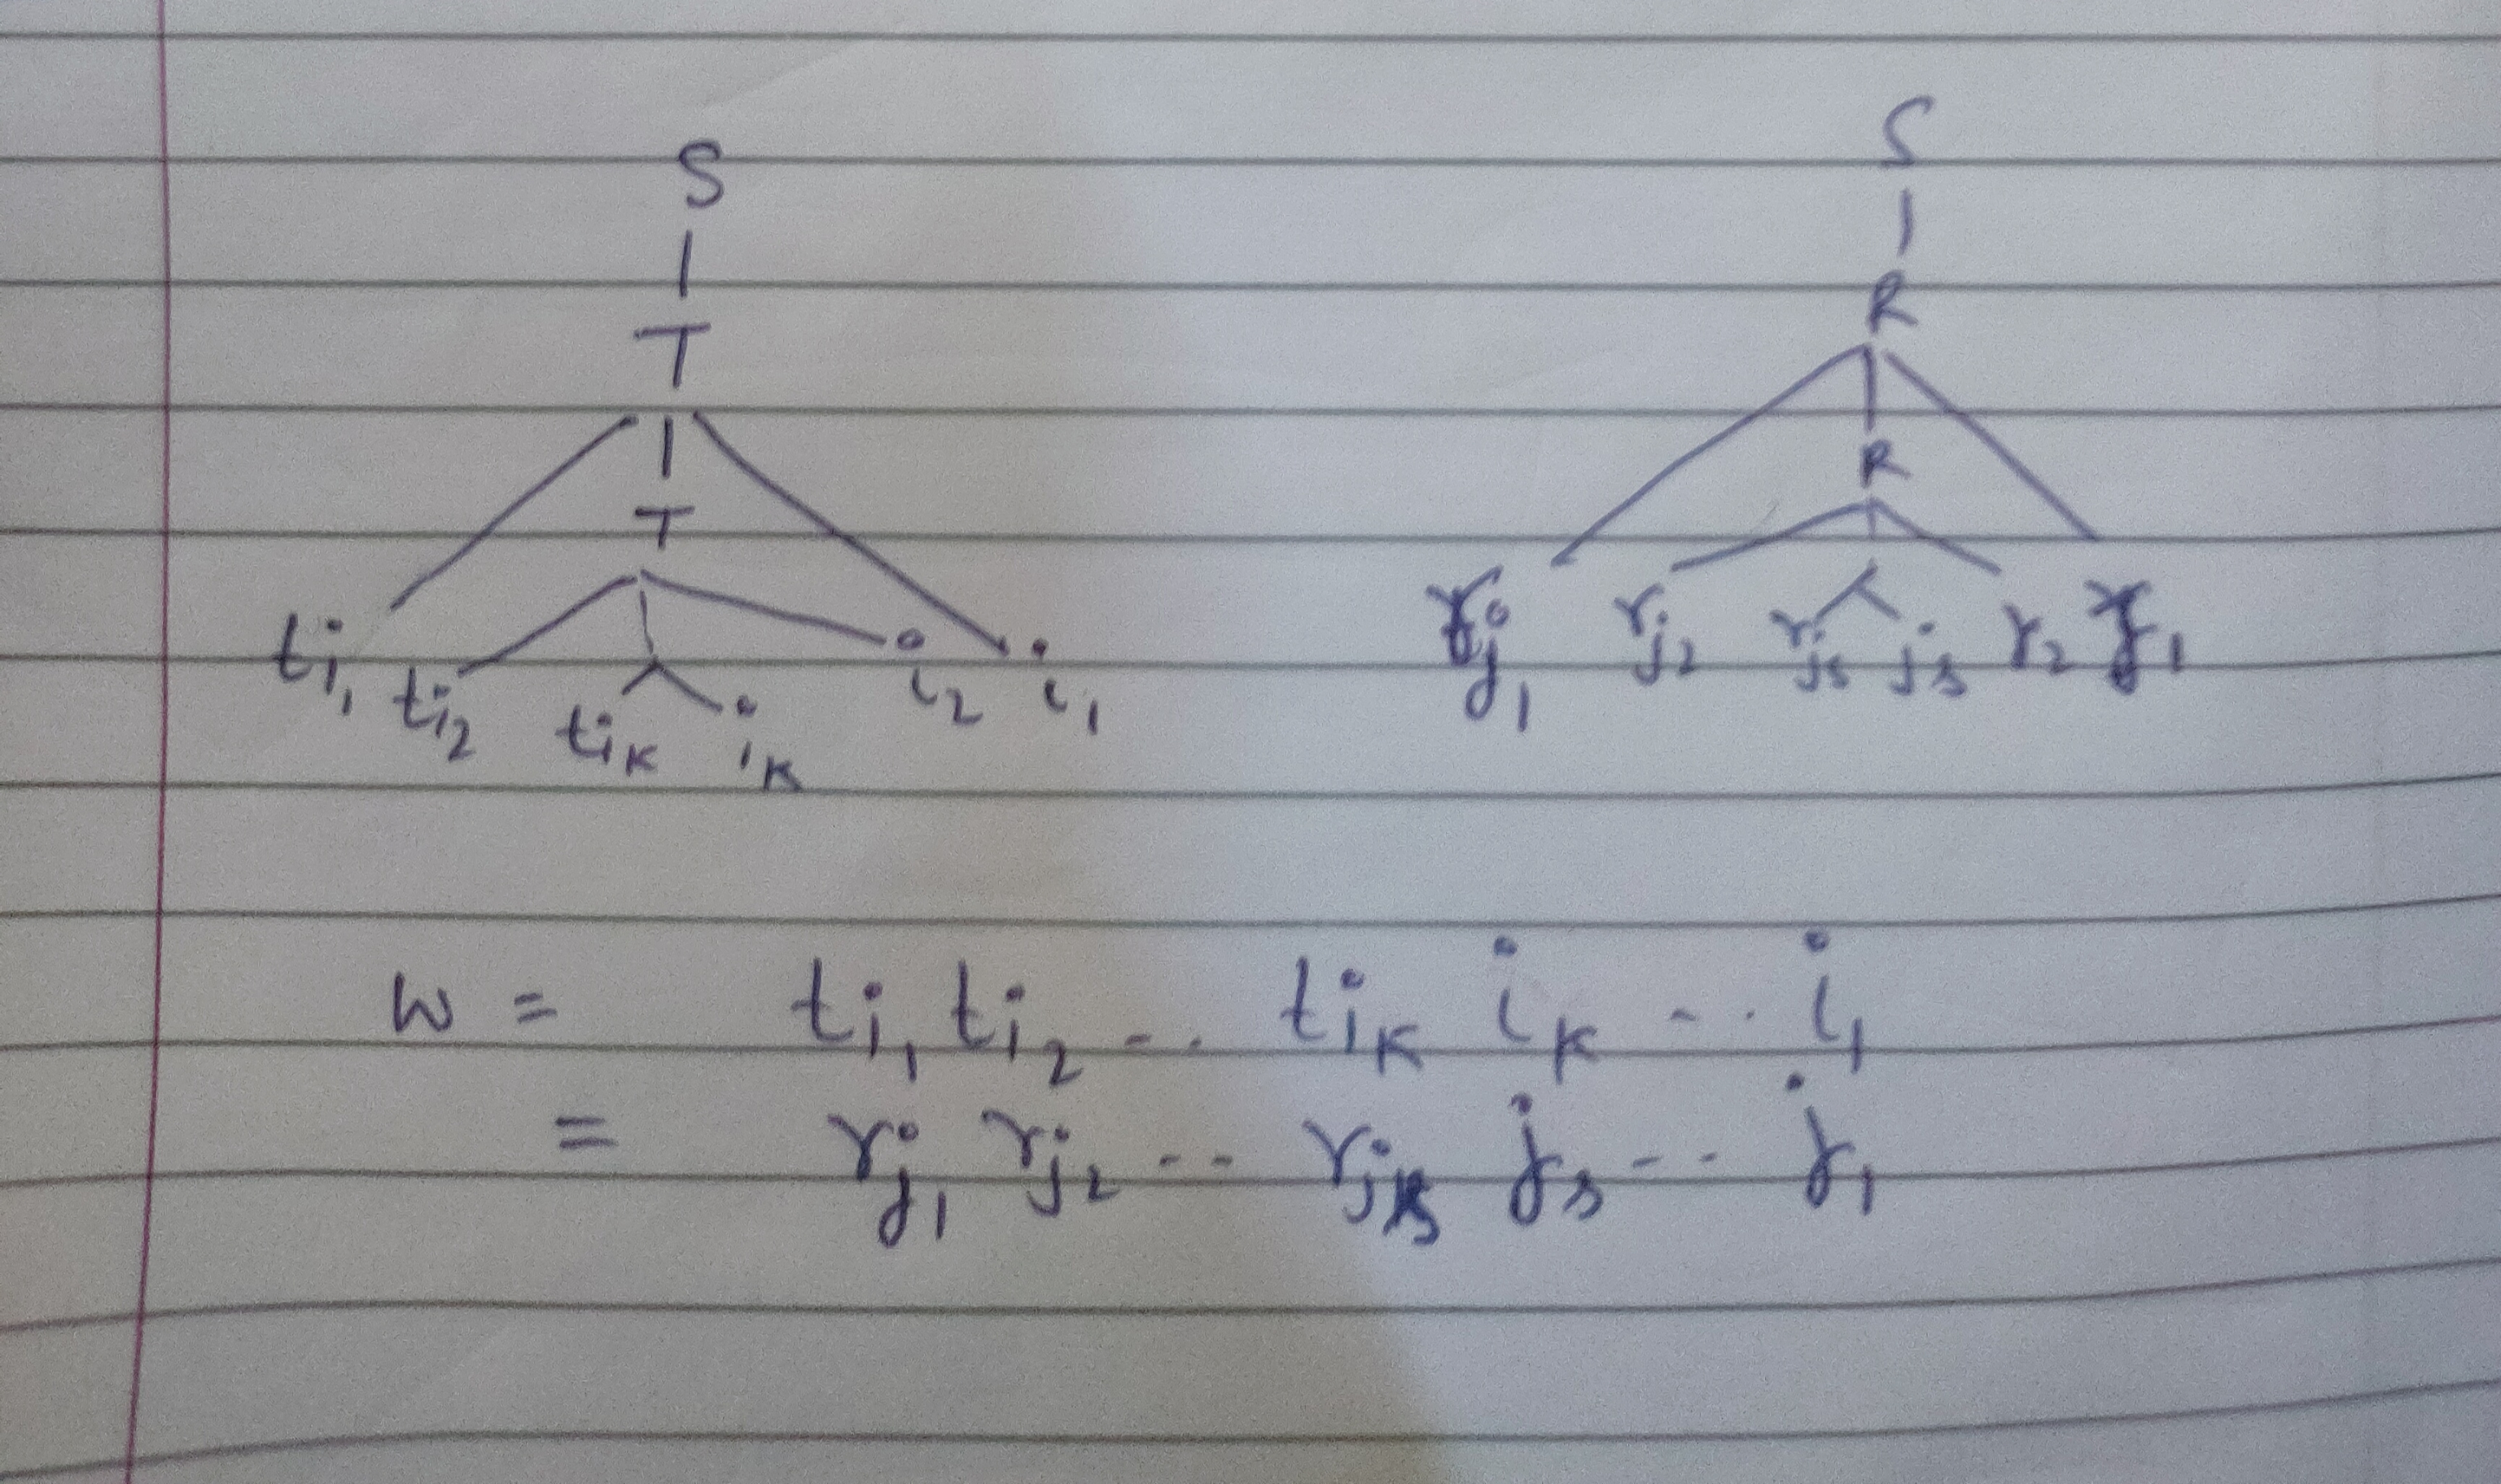
\includegraphics[width=7cm]{2.jpg}
    \end{figure}

    We have w = $t_{i_1}t_{i_2}....t_{i_k}i_k....i_1$ = $r_{j_1}r_{j_2}....r_{j_s}j_s....j_1$\\
    Matching frm last would give $i_1 = j_1 ..... i_k = j_s$ and also $k=s$ ----- (1)\\
    Matching remaining characters would yield $t_{i_1}t_{i_2}...t_{i_k} = r_{j_1}r_{j_2}....r_{j_s}$\\
    Using 1 gives:- \\
    $t_{i_1}t_{i_2}...t_{i_k} = r_{i_1}r_{i_2}....r_{i_k}$\\
    That is a solution of PCP.\\
\end{enumerate}
Hence if G is ambiguous then PCP is solvable. Moreover above proof with reverse implication can be used to prove that if G is unambiguous then PCP is not solvable. Because 
if G is unambiguous then there does not exist any such w each permutation of $t_i , r_i$ different.\\

Hence we have shown that solution of PCP can be found using $AM_{BCFG}$. More formally :- \\
Construct grammar G from any instance P of PCP.\\
Use $AM_{BCFG}$ to find whether G is ambiguous.\\
If G is ambiguous then accept .\\
Else reject.\\

This would imply that PCP is decidable but that is a contradiction hence $AM_{BCFG}$ is undecidable.\\

\pagebreak


\section{Question 8}
\textbf{In the Silly Post Correspondence Problem (SPCP), the top string in each pair has the same
length as the bottom string. Show that the SPCP is decidable.\\}

To prove that the SPCP is decidable we need to show that there exists a turing machine T that decides the SPCP.\\
We will provide a algorithm that can be implemented in a turing machine to decide the SPCP.\\

Now, lets first formally define the problem of SPCP.\\

\textbf{Given: }\\

$\lfloor \frac{t_1}{r_1} \rfloor , \lfloor \frac{t_2}{r_2} \rfloor ....... \lfloor \frac{t_n}{t_n} \rfloor$ \\
where, $t_i , r_i \in \Sigma^* , |t_i| = |r_i| \forall i \in [1,n]$\\

\textbf{To find: } \\
a sequence $\{ i_1,i_2.....i_k \}$ such that $t_{i_1}t_{i_2}.....t_{i_k} = r_{i_1}r_{i_2}.....r_{i_k}$\\

\textbf{The algorithm: }\\

First let us dicuss the approach informally, Now to find a sequence that satisfies above property, the first index $i_1$ should be chosen such that $t_{i_1}[0] = r_{i_1}[0]$ since we want the complete string to be same 
and for that first character must also be same.\\
Moreover, we want $t_{i_1}[0:k] = r_{i_1}[0:k]$ where k is $min(|t_{i_1}|,|r_{i_1}|)$\\
But we know that $|t_{i_1}| = |r_{i_1}|$\\
$ => t_{i_1} = r_{i_1}$ is needed for a solution to exists. ------ (1)\\
But if we have found such a index then we are done, since we have found a sequence = $\{i_1\}$  that satisfies the requirenment. That means existence of such an index is sufficient for the solution to exist\\
Also, existence of such a index is necessary for a solution to exist (from 1).\\
Hence to find the solution of SPCP we need to find an i such that $t_i = r_i$\\ That can be easily done by a turing machine without haulting.\\

For each $i \in [1,n]$ do\\
\hspace*{2cm} If $t_i = r_i$ then accept\\
\hspace*{0.5cm} If no such i exist then reject\\

\pagebreak



\end{document}

